% Final Report
% The final reports should be in the style of a short research paper of three pages (about one page text plus plots & figures).
% The format for the report has to be the standard IEEE conference format: https://www.ieee.org/conferences/publishing/templates.html

\documentclass[conference]{IEEEtran}
\usepackage{amsmath,amssymb,amsfonts}
\usepackage{algorithmic}
\usepackage{cite}
\usepackage{bm}
\usepackage{graphicx}
\usepackage{textcomp}
\usepackage{xcolor}
\usepackage[caption=false,font=footnotesize]{subfig}

% \usepackage{subcaption}
% \captionsetup{compatibility=false}


\def\BibTeX{{\rm B\kern-.05em{\sc i\kern-.025em b}\kern-.08emT\kern-.1667em\lower.7ex\hbox{E}\kern-.125emX}}


\begin{document}


\title{Neural Networks for \\Inverse Kinematics Problems in Robotics}

\author{\IEEEauthorblockN{Franziska Schwaiger}
    \IEEEauthorblockA{\textit{Matriculation number: 03658670}}
    \and
    \IEEEauthorblockN{Thomas Barthel Brunner}
    \IEEEauthorblockA{\textit{Matriculation number: 03675118}}
}

\maketitle

\section*{Introduction}

In our project, we are evaluating the feasibility of using neural networks in robotics. More specifically, we are investigating the performance of Invertible Neural Networks (INN) and Conditional Variational Autoencoders (cVAE) for learning the inverse kinematics of a planar robotic arm with revoulte joints. In this report, we outline the progress made and discuss the results we have obtained.

\section*{Methods}
\subsection*{Robot Simulations}

To evaluate the performance of the architectures, we developed simulations of planar robotic arms with revolute joints for an arbitraty number of degrees of freedom (DoFs). In general, the forward kinematics equations of a planar robot arm with link lengths \( l_i \) and \( N \) revolute joints with joint angles \( \theta_i \in [-\pi, \pi] \) can be described as:
\begin{equation}
    x_\text{TCP} = \sum_{i=1}^{N}{l_i \cos\left( \sum_{j=1}^{i}{\theta_j} \right)}, \ 
    y_\text{TCP} = \sum_{i=1}^{N}{l_i \sin\left( \sum_{j=1}^{i}{\theta_j} \right)}
\end{equation}

To improve the training and testing performance of our models, we modified these equations for fast vectorized numerical computation. The resulting operations and be seen in Equation~\ref{tcp vectorized}, with joint angles vector \( \bm{\theta} = \left[ \theta_1, \theta_2 , ... \right]^\text{T} \), the upper triangular matrix with ones as elements \( \bm{U} \) and the link lengths vector \( \bm{l} = \left[ l_1, l_2, ... \right]^\text{T} \).
\begin{equation}
    x_\text{TCP} = \cos \left( \bm{\theta}^\text{T}\ \bm{U} \right) \bm{l}, \ 
    y_\text{TCP} = \sin \left( \bm{\theta}^\text{T}\ \bm{U} \right) \bm{l}
    \label{tcp vectorized}
\end{equation}

In our current setup, we do not take the angle of the tool center point (TCP) into consideration. Thus, the location of the TCP is defined by its \( x, y \) coordinates. As a result of this, all simulations with more than 2 DoF can have up to infinite solutions of the inverse kinematics for a given TCP position. The 2 DoF robot arm can have up to two solutions.

\subsection*{Dataset}

We generated four different datasets for different robot configurations. Each dataset is composed of \( 10^6 \) samples of robot configurations and corresponding TCP coordinates. In our experiments, we used simulations with 4, 6, 8 and 10 DoF. Each configuration was sampled from a normal distribution \( \theta_i \sim \mathcal{N}(\mu=0, \sigma=0.2) \). Thus, the dataset is composed mostly of configurations in which the robot arm is extended. This reflects real-world use cases of robot arms, which have limited workspaces and whose tasks are focused on one section of the workspace. Moreover, limiting the range of the joints improved the performance of the networks, as it simplifies the problem and as it avoids the discontinuity in the angles at \( \theta = \pm \pi \). Figure~\ref{fig:datasets} shows an illustration of the datasets. 

\begin{figure}[ht]
    \centering
    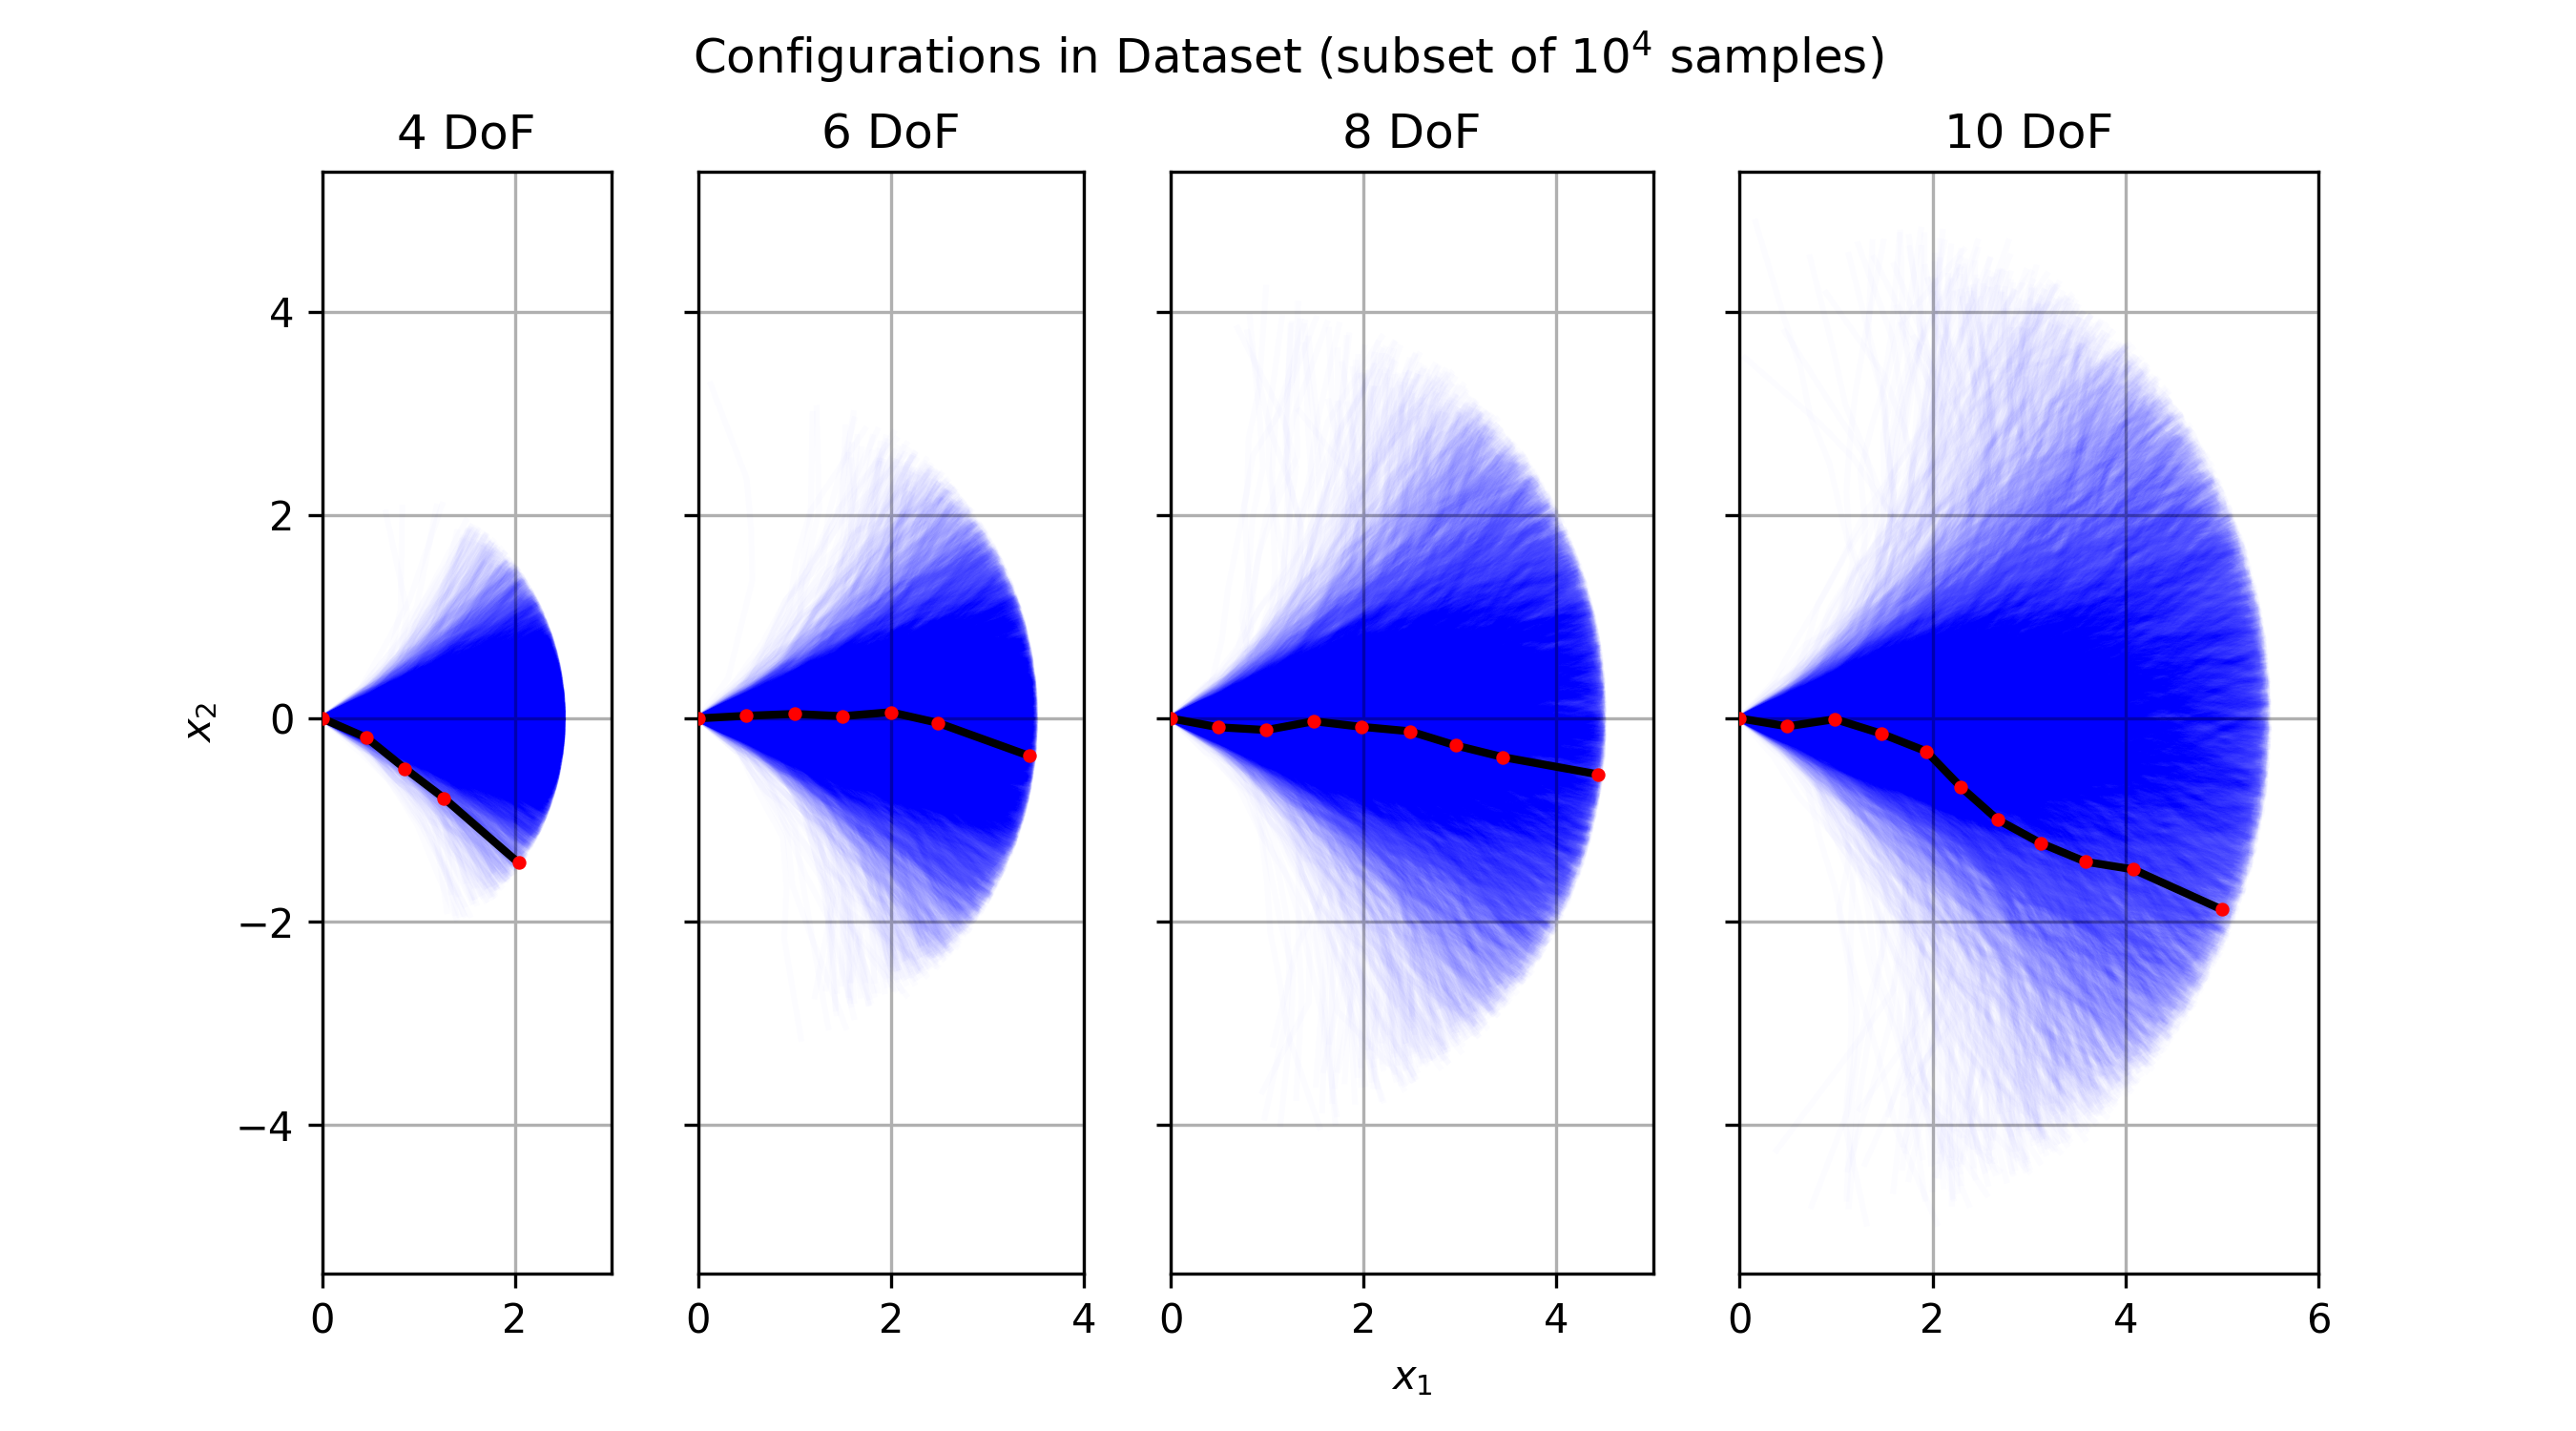
\includegraphics[width=\linewidth]{figures/normal_std_0_2_all_DoF.png}
    \caption{Illustration of a subset of the datasets (\( 10^4 \) samples) of the robot configurations.}
    \label{fig:datasets} 
\end{figure}

\subsection*{Considering Singularities}

As was already mentioned in the previous section, we avoid discontinuities by restricting the configuration space of the robot. Yet we implemented two approaches which consider this discontinuity in the angles at $\theta_i = \pm \pi$ to extend the implemented networks to inverse kinematics problems with general configuration spaces.

The first approach is a non-minimal parameterization of the configuration space that uses an augmented vector-based representation of the angles, which was already described in the midterm report. The drawback of this approach is its larger input space, which makes the task increasingly harder to solve for robots with higher DoFs.

For this reason, we also considered an alternative approach, in which we the discontinuities are considered in the loss function of the reconstruction error. It ensures that the computation of distances between angles takes the orientation of these angles into consideration. Thus, it avoids large negative losses for angles with distinct values, but whose orientation is similar.

\subsection*{Network Architectures}

As described in the midterm report, we implemented and investigated two network architectures for generating the full posterior distribution of the joint angles: conditional Variational Autoencoders and Invertible Neural Networks. 

Unlike Variational Autoencoders (VAE) \cite{Kingma2014}, conditional Variational Autoencoders (cVAE) \cite{Sohn2015} are able to control the data generation process by conditioning the latent space $z$. Considering the application of inverse kinematics, samples are drawn from $p(z) \sim N(0, 1)$ and the predicted posterior distribution of the joint angles is then generated conditioned on the end-effector position.

Invertible Neural Networks (INN) \cite{Ardizzone2018} model a bijective mapping from the joint angles to the end-effector position by stacking invertible blocks together. Here, the dimensionality of the joint angles $x$ is the same as the concatenated output consisting of the latent space $z$ and the end-effector position $y$. The predicted posterior of the joint angles is then generated similar to cVAE by sampling from $p(z) \sim N(0, 1)$ and then running the network backwards conditioned on $y$.

Additionally, INNs share properties with normalizing flows \cite{normalizingFlows2010, normalizingFlows2013} which gradually transform a normal density into the desired data density. They are also bijective and for both normalizing flows and INNs, a tractable Jacobian exists which allows explicit computation of posterior probabilities. As the focus in this work lies on the comparison between cVAE and INN, normalizing flows are not considered anymore.

As stated in \cite{Ardizzone2018}, INNs only need to be trained on the well-understood forward process. The inverse process can be obtained for free by just running the network backwards at prediction time. The authors also mention that results can be improved with additional unsupervised backward training. When applying INNs to the inverse kinematics problem, we found that unsupervised backward training is crucial to match the performance of the cVAE. This results in two network passes per training step to accumulate the gradients, which leads to much slower training. Additionally, when training INNs the parameters need to be adjusted carefully as training can become unstable.

\subsection*{Hyperparameter Optimization}

As stated before, we trained a network of each architecture (cVAE and INN) for each dataset (4, 6, 8 and 10 DoF), which resulted in 8 models with different complexities. The sizes and hyperparameters of each model had to match the complexity of the simulation. To compare the performance of the networks across different DoFs in a fair setting, we used Tune \cite{liaw2018tune} and Scikit Optimize \cite{scikit-optimize} to perform a black-box optimization of the hyperparameters. For each model, 100 sets of hyperparameters were sampled, which were then used to train the networks using a subset of the main dataset (\( 10^4 \) samples). We opted for a reduced number of samples to help reduce the computation time of the hyperparameter search. 

For the cVAE, we optimized the learning rate, the weight decay, the number of hidden layers for the encoder and decoder and the amount of neurons per layer. For the INN, we optimized the learning rate, the weight decay, the number of coupling layers, the amount of layers per subnet and also the number of neurons per subnet layer. The ranges of hyperparameters used can be seen in Tables~\ref{tab:hyperparameter-ranges-inn} and \ref{tab:hyperparameter-ranges-cvae}. These values were based on intuition and previous experience in training these networks.

\begin{table*}[ht]
    \caption{Ranges of inn hyperparameters used during hyperparameter search.}
    \label{tab:hyperparameter-ranges-inn}
    \centering
    \begin{tabular}{|l|c|c|c|c|c|}
    \hline
      & Learning rate & \# Subnet layers & \# Coupling layers & \# Neurons per layer & Weight decay \\
     \hline
     Min  & 0.0001 & 3 & 6 & 100 & 0.00001 \\
     Max  & 0.005 & 7 & 10 & 300 & 0.001 \\
     \hline
    \end{tabular}
\end{table*}

\begin{table*}[ht]
    \caption{Ranges of cvae hyperparameters used during hyperparameter search.}
    \label{tab:hyperparameter-ranges-cvae}
    \centering
    \begin{tabular}{|l|c|c|c|c|}
    \hline
      & Learning rate & \# Layers & \# Neurons per layer & Weight decay \\
     \hline
     Min  & 0.0001 & 3 & 200 & 0.00001 \\
     Max  & 0.01 & 15 & 500 & 0.001 \\
     \hline
    \end{tabular}
\end{table*}

\subsection*{Implementation}

The previous two model architectures (cVAE and INN) have been implemented in PyTorch and are inspired by existing implementations in  \cite{graviraja2019, freia2020}. We used the Google Compute Engine to perform the hyperparameter search and to train our models.

\section*{Experimental Evaluation}

\subsection*{Evaluation protocol}

We trained each model using the best performing hyperparameters from the hyperparameter search. In total, we have four INN and four cVAE models, each corresponding to a different simulation (4, 6, 8 or 10 DoF). The batch size used during training was $1000$ for both network architectures. All models were trained for 60 epochs on a dataset with 1 million samples and a train and test split of 70\% and 30\%, respectively. For evaluating the performance of each model, we used two evaluation metrics which have already been described in the midterm report and in \cite{Kruse2019}:

1. The average posterior mismatch between the distribution generated by the model and the ground truth estimate obtained via rejection sampling. For generating the posterior, we used 100 samples per ground truth position and averaged over 1000 samples from the test dataset.

2. The average re-simulation error as the mean squared distance between the ground truth end-effector position and the re-simulated end-effector position obtained from the predicted joint angles. The re-simulation error was averaged over the whole test dataset.

\subsection*{Results}

%%%%%%%%%%%%%%%%%%%%%%
% TABLES
%%%%%%%%%%%%%%%%%%%%%%
\begin{table*}[h]
\caption{Best-performing hyperparameters for cvae trained on a planar robot with revolute joints}
\label{tab:results:cvae}
\centering
\begin{tabular}{|c|c|c|c|c|c|}
\hline
DoF & Learning rate & \# Layers & \# Neurons per layer & Weight decay & \# Trainable parameters \\
\hline
4  & 0.009 & 3 & 230 & 0.0002 & 217128 \\
6  & 0.0041 & 3 & 200 & 0.00001 & 166814 \\
8  & 0.0001 & 3 & 500 & 0.00001 & 1022020 \\
10  & 0.00063 & 5 & 400 & 0.00029 & 1303226 \\
\hline
\end{tabular}
\end{table*}

\begin{table*}[h]
\caption{Best-performing hyperparameters for inn trained on a planar robot with revolute joints}
\label{tab:results:inn}
\centering
\begin{tabular}{|c|c|c|c|c|c|c|c|}
\hline
DoF & Learning rate & \# Subnet layers & \# Coupling layers & \# Neurons per layer & Weight decay & \# Trainable parameters \\
\hline
4  & 0.0009 & 5 & 9 & 100 & 0.00008 & 1108872 \\
6  & 0.001 & 5 & 7 & 180 & 0.0003 & 2772084 \\
8  & 0.0014 & 4 & 9 & 115 & 0.0004 & 997884 \\
10  & 0.002 & 5 & 7 & 170 & 0.0005 & 2494380 \\
\hline
\end{tabular}
\end{table*}

The best performing hyperparameters from the hyperparameter search for the cVAE and INN are shown in Tables~\ref{tab:results:cvae} and \ref{tab:results:inn}, respectively. Due to the hyperparameter search, the number of parameters of the models differ by a large amount. As it can be seen in the tables, the best performing models are not the ones with the greatest number of trainable parameters. This serves to show that the hyperparameters search space is sufficient. 

The results of the evaluations (the mismatch of the posterior distribution and the re-simulation error) are plotted over the number of parameters in Figures~\ref{fig:plot:posterior} and \ref{fig:plot:resim}, respectively. Each plotted point is labelled with the corresponding DoF. From Figure~\ref{fig:plot:posterior} we can see that the mismatch of the predicted posterior with the ground truth posterior obtained from rejection sampling is smaller for the INN when compared with the cVAE. However, as seen in Figure~\ref{fig:plot:resim}, the cVAE performs consistently better on the re-simulation error when compared with the INN.

%%%%%%%%%%%%%%%%%%%%%%
% RESULTS, FIGURES
%%%%%%%%%%%%%%%%%%%%%%
\begin{figure}[ht]
\centering
	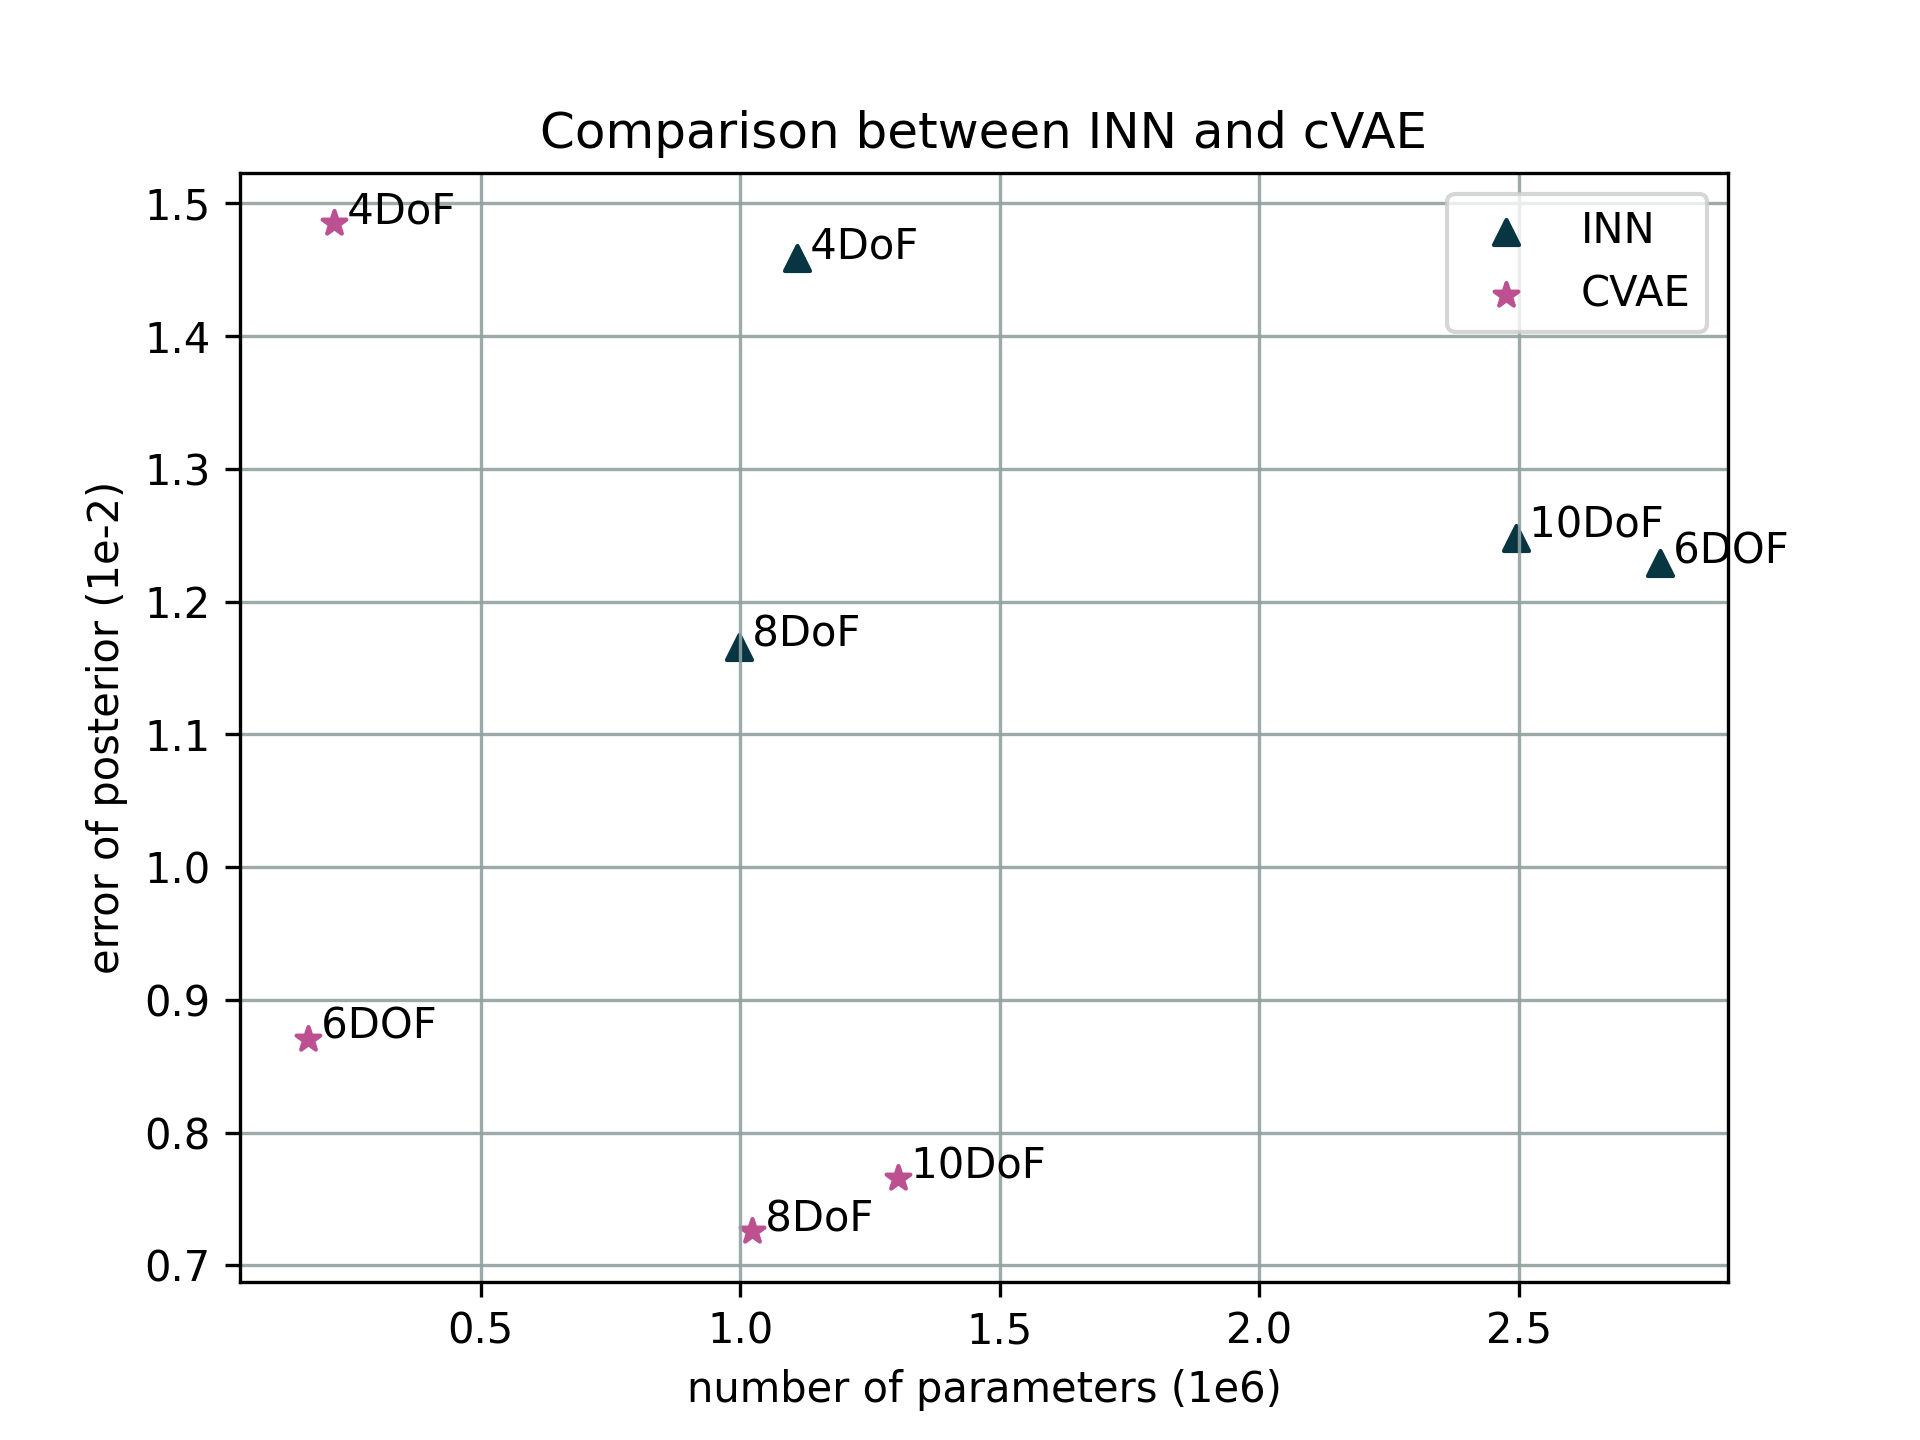
\includegraphics[width=\linewidth]{figures/comparison_e_posterior_alternative.png}
    \caption{\label{fig:plot:posterior} Average posterior mismatch between the distribution generated by the model and the ground truth estimate obtained via rejection sampling.}
\end{figure}

\begin{figure}[ht]
\centering
	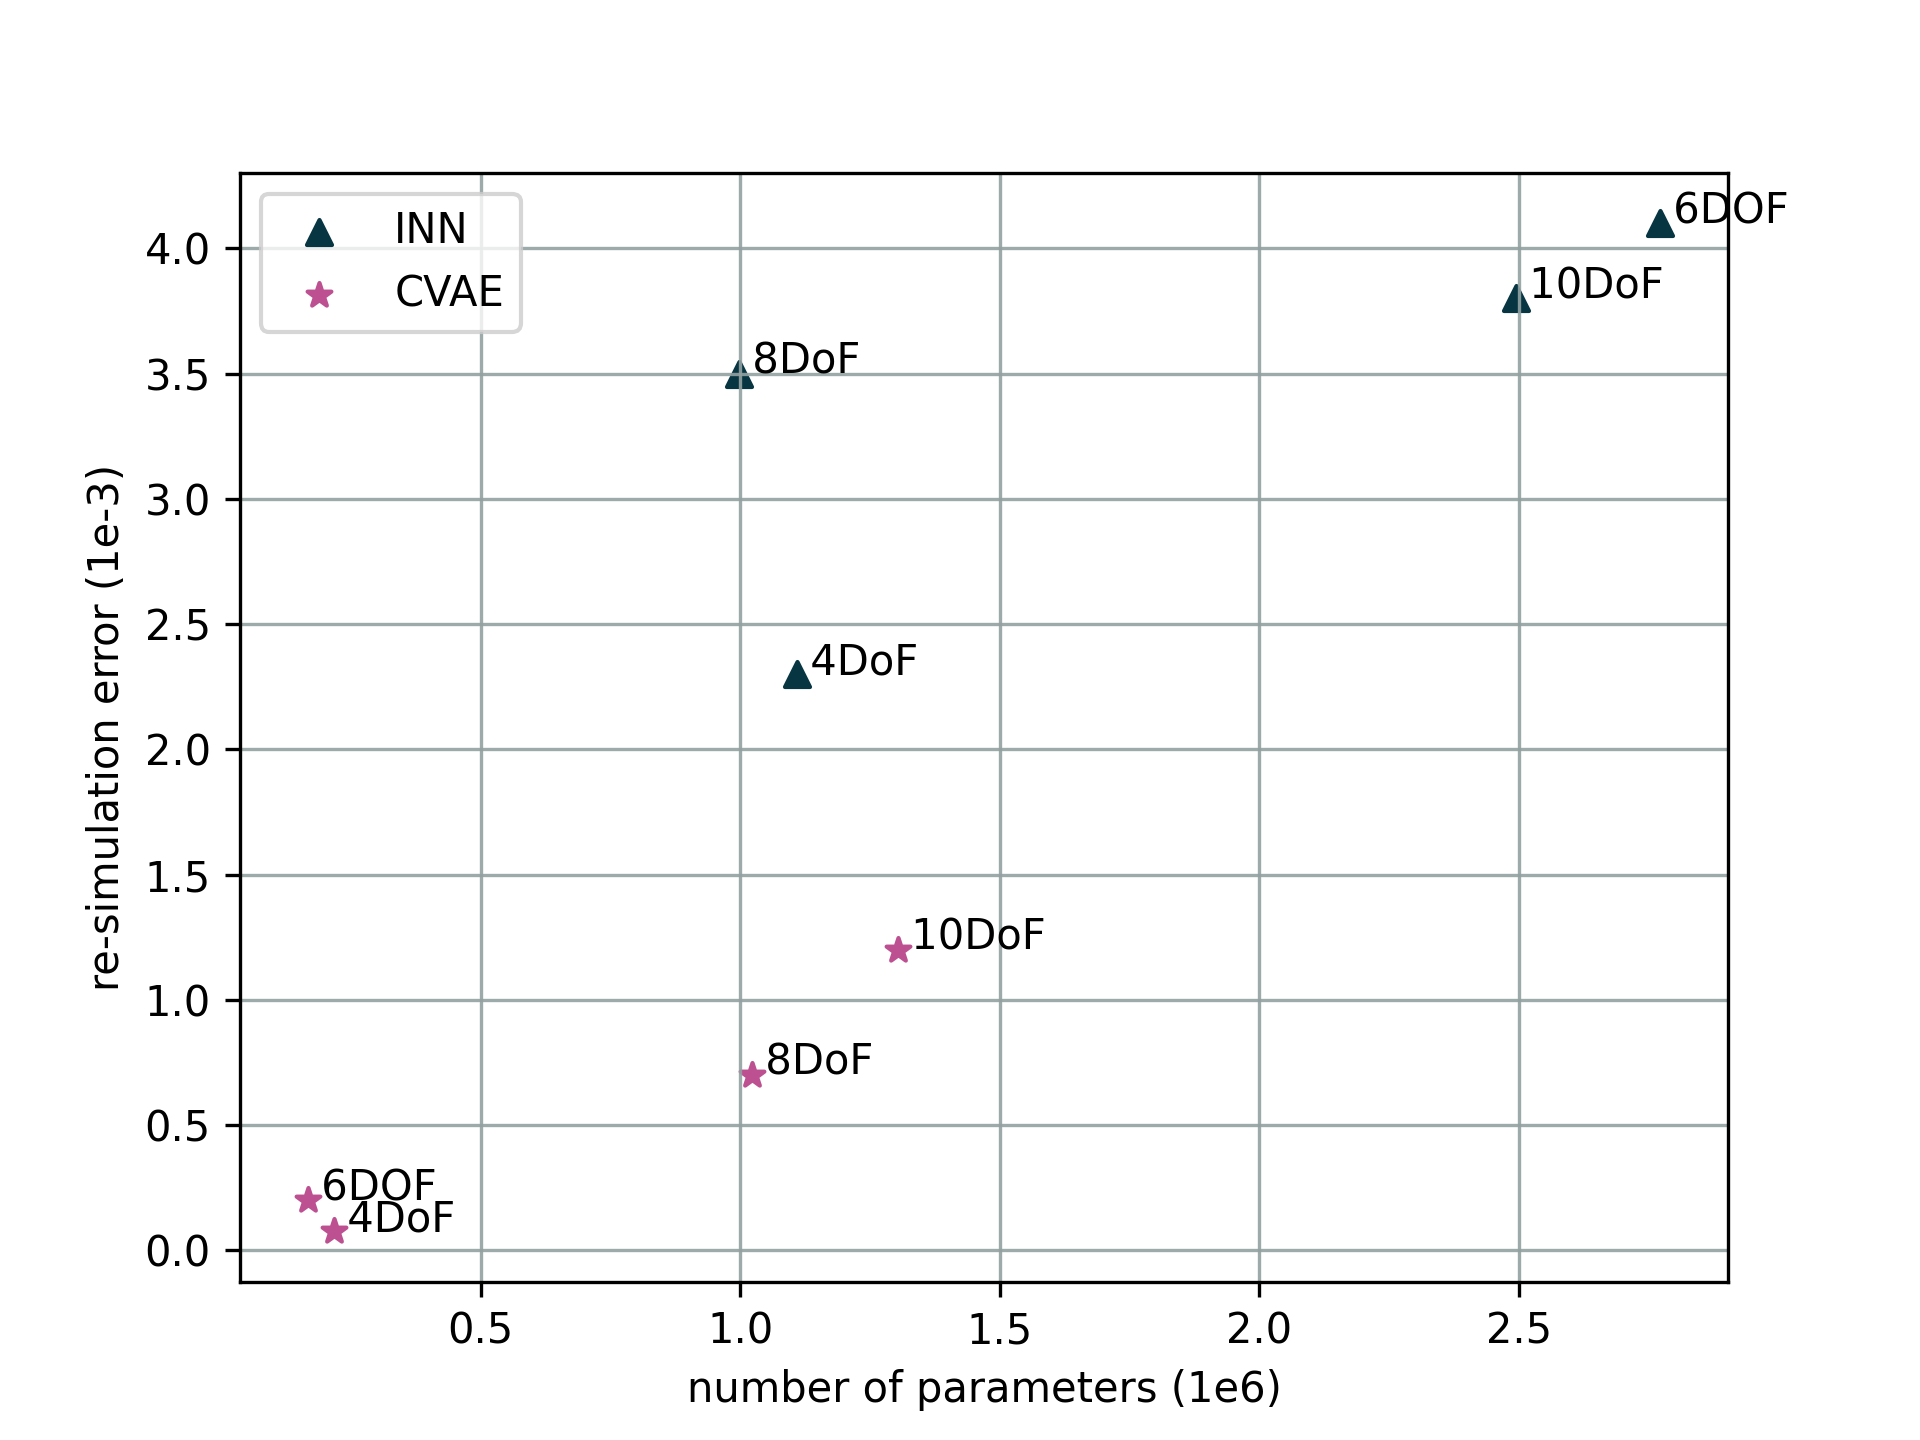
\includegraphics[width=\linewidth]{figures/comparison_e_resim_alternative.png}
    \caption{\label{fig:plot:resim} Average re-simulation error as the mean squared distance between the ground truth end-effector position and the re-simulated end-effector position obtained from the predicted joint angles.}
\end{figure}

These results are illustrated in more detail with examples of 6DoF and 10DoF robots in Figures~\ref{fig:q_quantile:6DOF} and \ref{fig:q_quantile:10DOF}. A convex hull is drawn around the 97th percentile of the re-simulated points (green dots) and the corresponding ground truth end-effector position (red dot) for the cVAE and INN, respectively.  As it can be seen, the area of this convex hull is larger for the INN ($0.43$ / $1.15$) when compared with the cVAE ($0.15$ / $1.02$). But despite of having a larger re-simulation error, the INN generates the full posterior distribution of the joint angles much better than the cVAE, as can be seen in Figures~\ref{fig:posterior:6dof} and \ref{fig:posterior:10dof} for the 6DoF and 10 DoF robot, respectively. 

%%%%%%%%%%%%%%%%%%%%%%
% FIGURES, CONVEX HULL
%%%%%%%%%%%%%%%%%%%%%%
\begin{figure*}[tbh]
\centering
	\subfloat[cVAE]{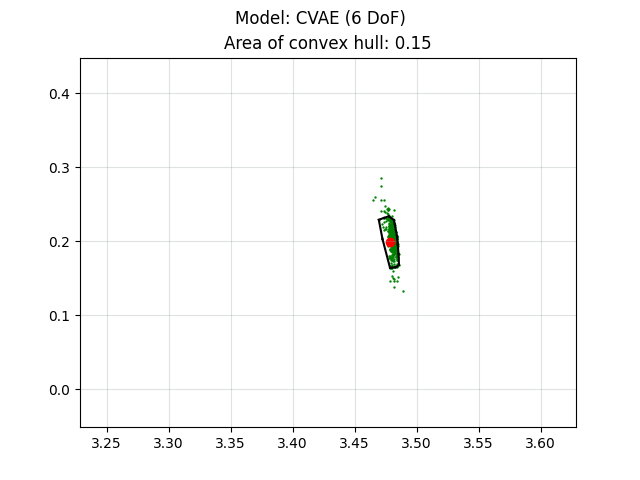
\includegraphics[width=0.47\linewidth]{figures/q_quantile_prediction_CVAE_6DOF.png}
        \label{fig:q_quantile:cVAE:6DOF}}
    %
    \subfloat[INN]{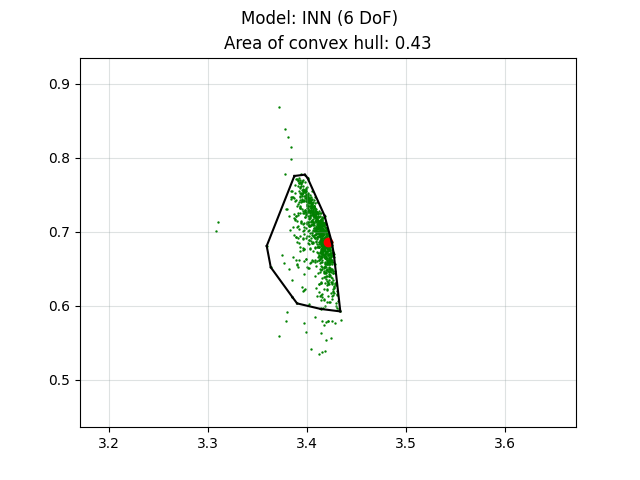
\includegraphics[width=0.47\linewidth]{figures/q_quantile_prediction_INN_6DOF.png}
        \label{fig:q_quantile:INN:6DOF}}

    \caption{Area of the convex hull of the \(97\)th percentile of the re-simulated end-effector coordinates with the ground truth end-effector position at $(x, y) = [3.42, 0.68]$ and $1000$ samples for a robot simulation with 6 DoF.}
    \label{fig:q_quantile:6DOF}
\end{figure*}

\begin{figure*}[tbh]
\centering
	\subfloat[cVAE]{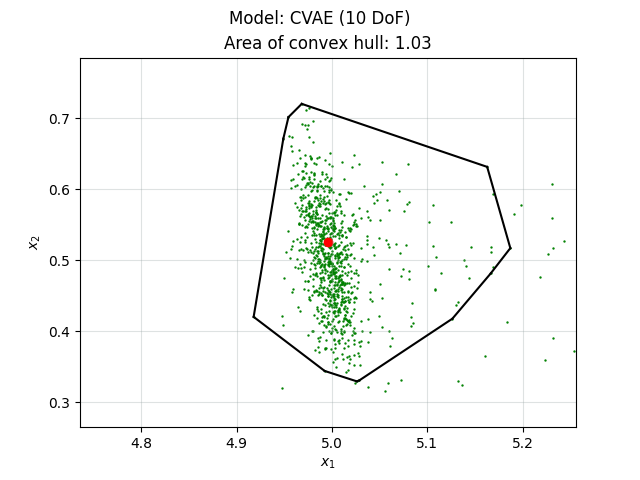
\includegraphics[width=0.47\linewidth]{figures/q_quantile_prediction_CVAE_10DOF.png}
    \label{fig:q_quantile:cVAE:10DOF}}
    %
    \subfloat[INN]{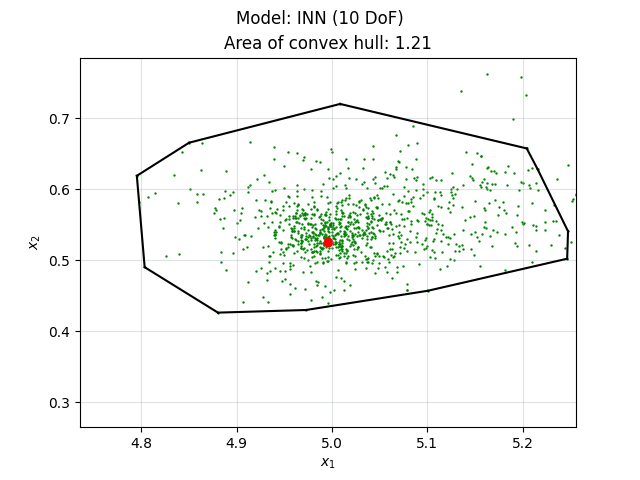
\includegraphics[width=0.47\linewidth]{figures/q_quantile_prediction_INN_10DOF.png}
        \label{fig:q_quantile:INN:10DOF}}

    \caption{Area of the convex hull of the \(97\)th percentile of the re-simulated end-effector coordinates with the ground truth end-effector position at $(x, y) = [5.00, 0.53]$ and $1000$ samples for a robot simulation with 10 DoF.}
    \label{fig:q_quantile:10DOF}
\end{figure*}
%%%%%%%%%%%%%%%%%%%%%%
% FIGURES, POSTERIOR
%%%%%%%%%%%%%%%%%%%%%%

\begin{figure*}[tbh]
\centering
	\subfloat[Rejection Sampling]{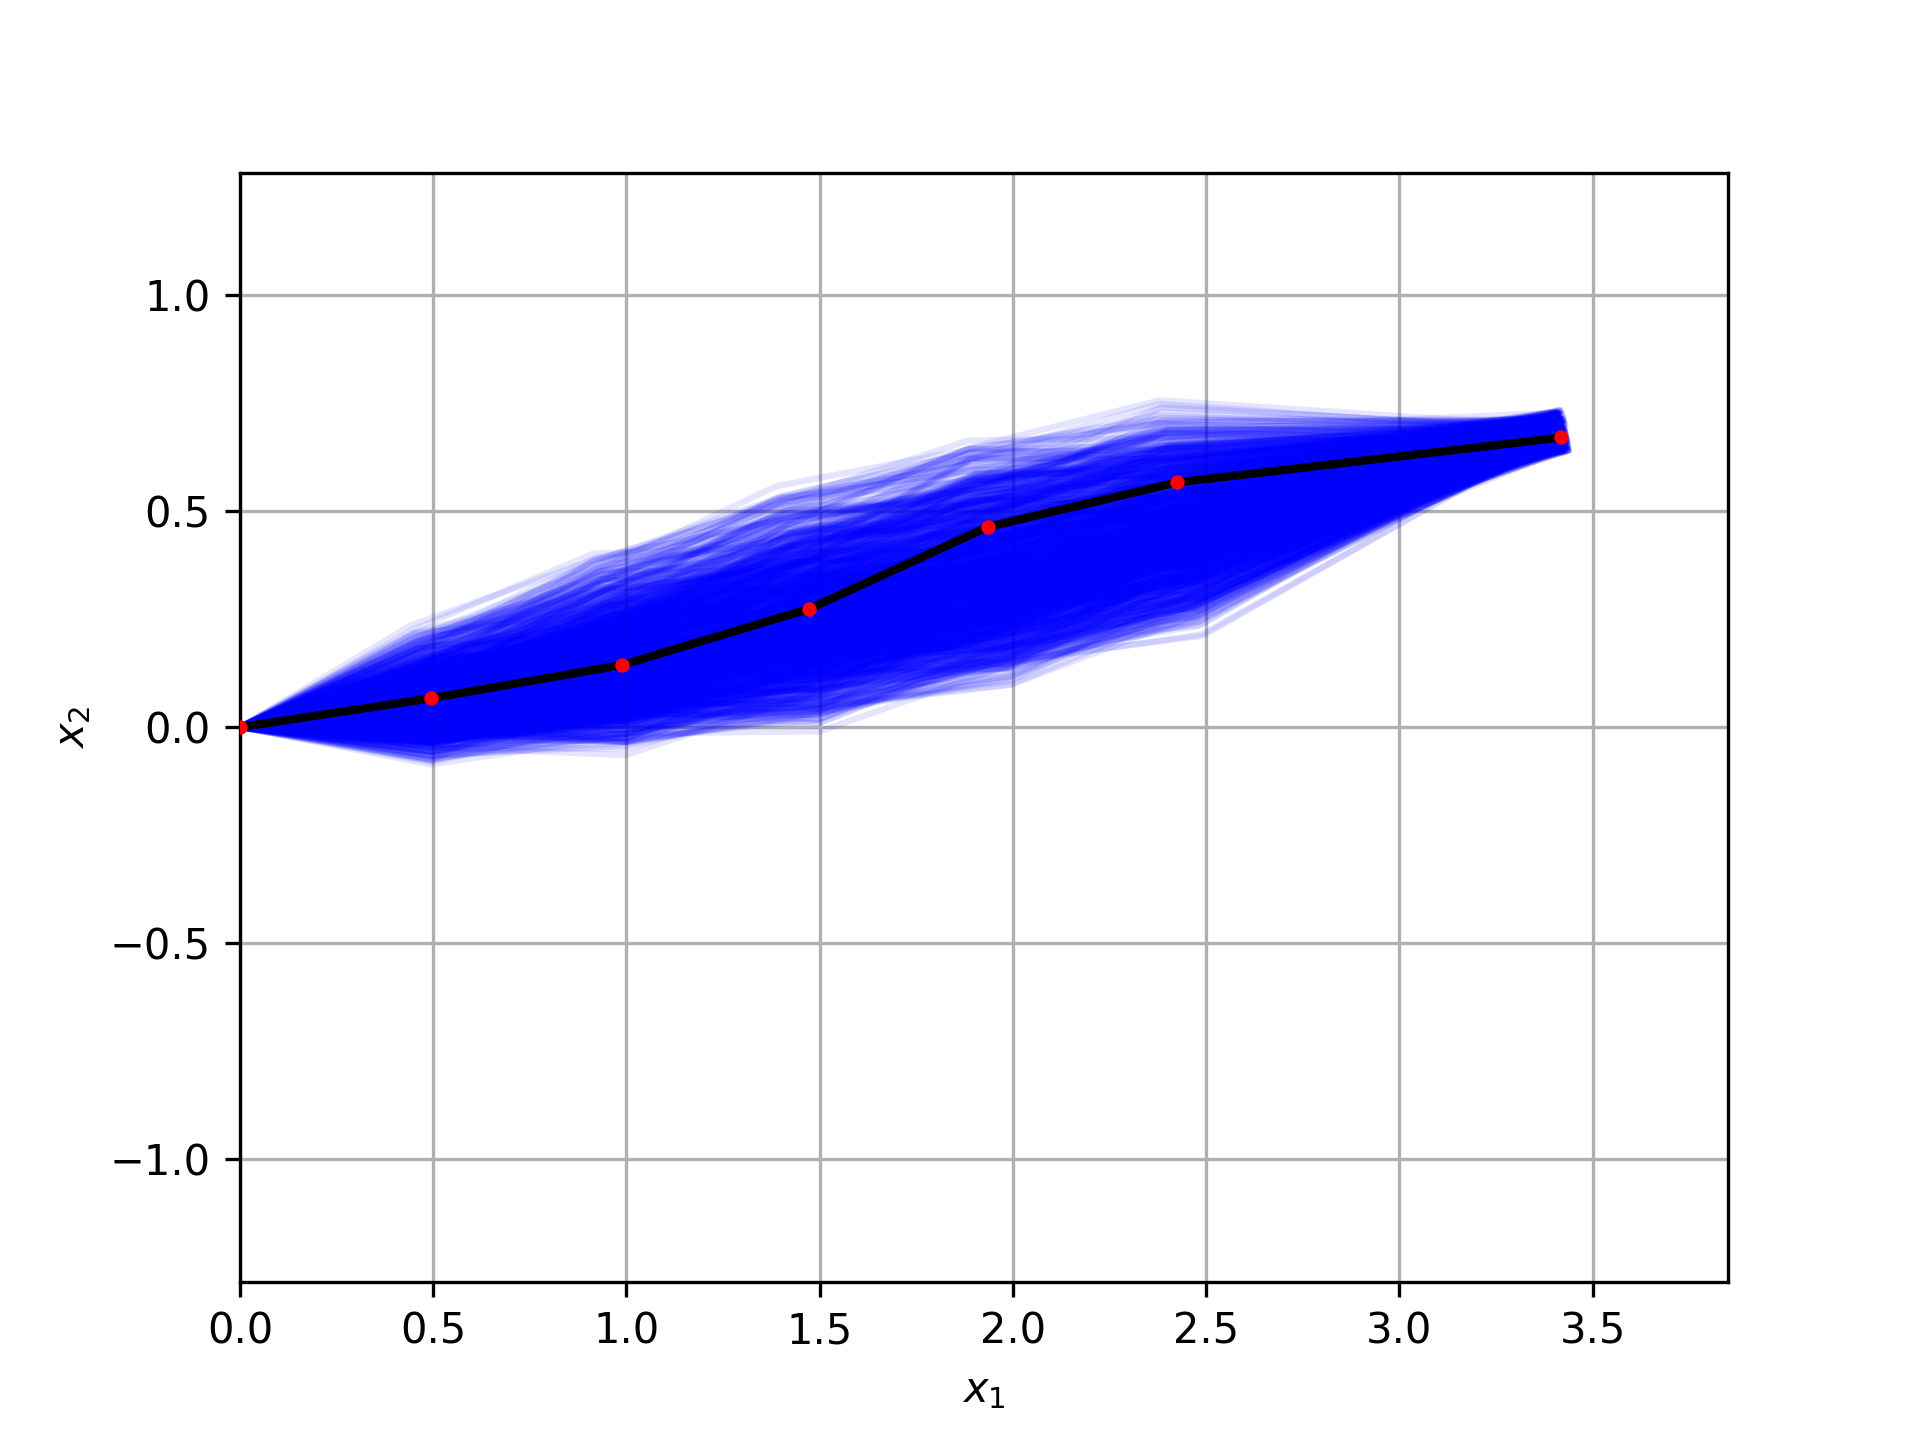
\includegraphics[width=0.32\linewidth]{figures/rejection_sampling_INN_6DOF.png}
    \label{fig:rejection_sampling:6DOF}}
    %
    \subfloat[cVAE]{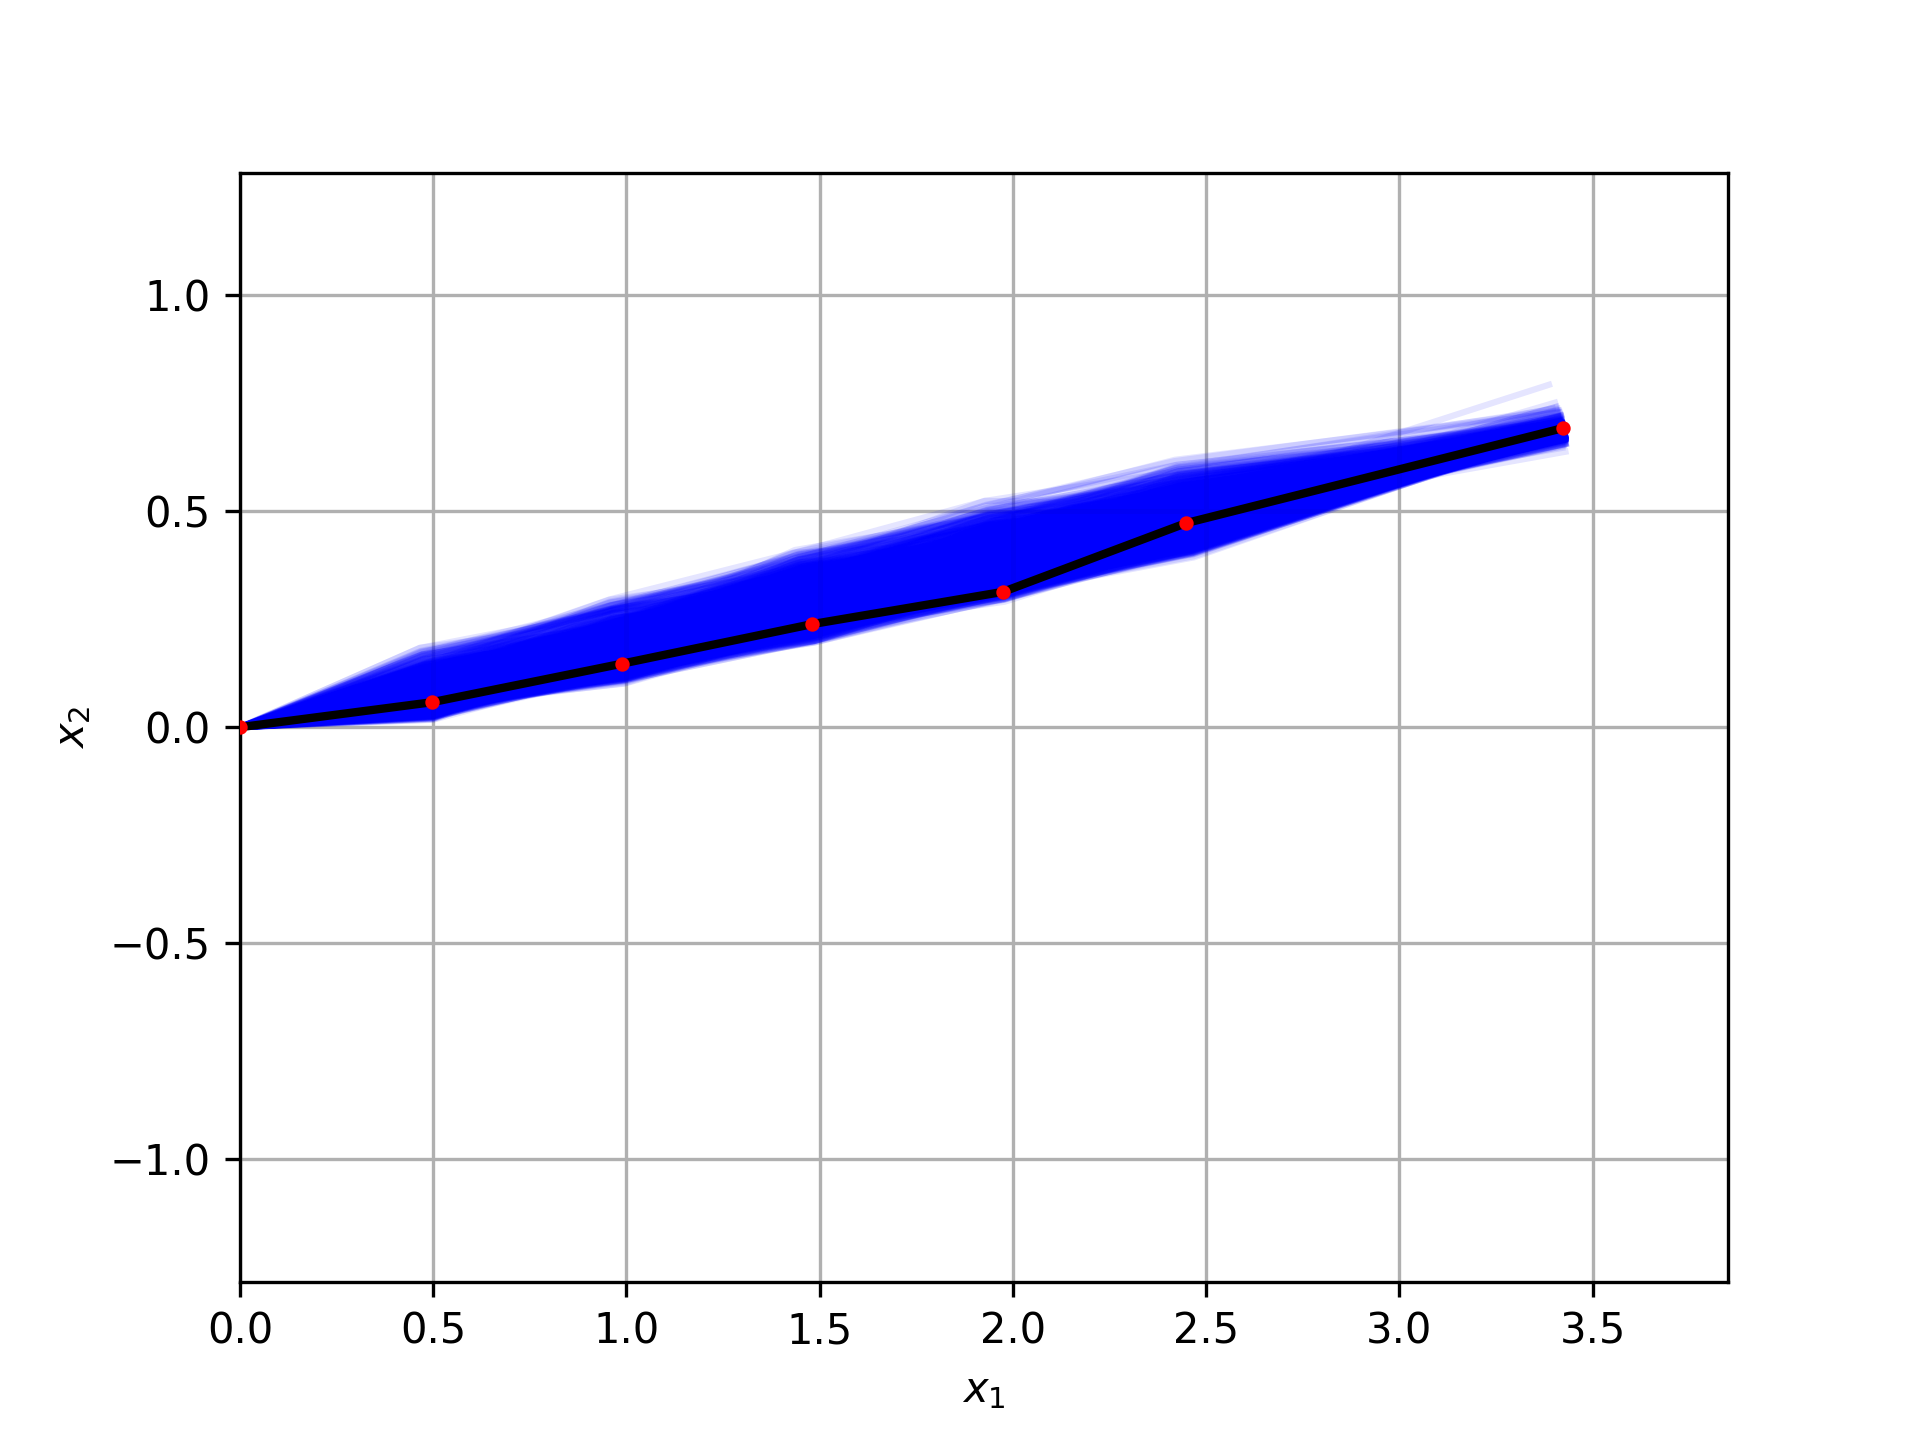
\includegraphics[width=0.32\linewidth]{figures/predicted_posterior_CVAE_6DOF.png}
        \label{fig:cVAE:6DOF}}
    %
    \subfloat[INN]{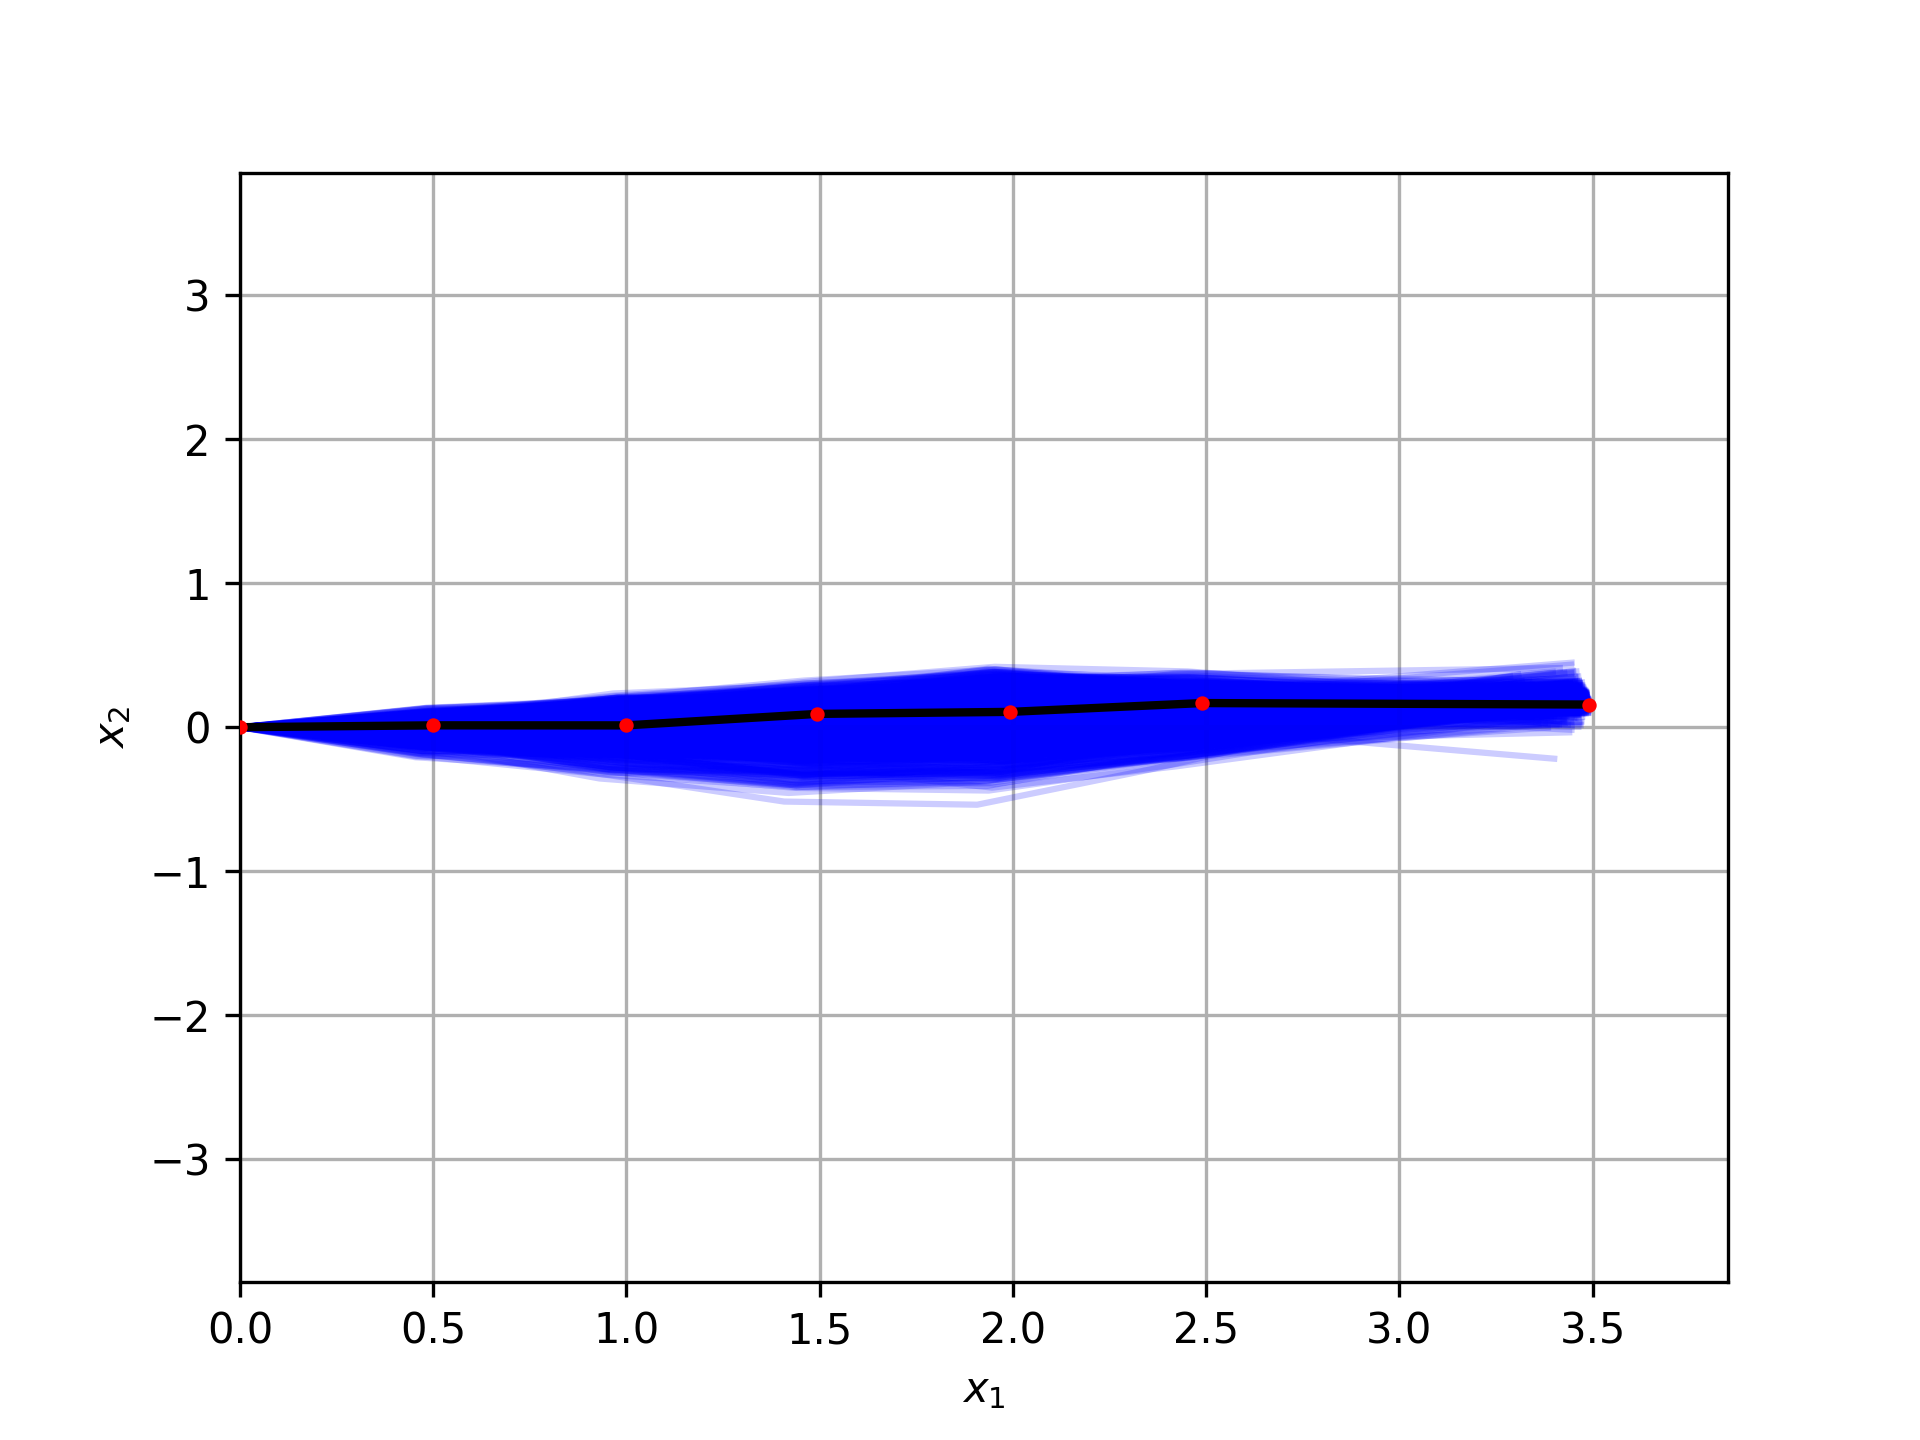
\includegraphics[width=0.32\linewidth]{figures/predicted_posterior_INN_6DOF.png}
        \label{fig:INN:6DOF}}

    \caption{Configurations of a planar manipulator with $6$ revolute joints and end-effector position at $(x, y) = [3.42, 0.68]$. 1000 samples are drawn from each model's predicted posterior $\tilde{p}(x | y_{gt})$. One random sample configuration is highlighted. $e_{posterior} = 0.012$ for the cVAE and $e_{posterior} = 0.0068$ for the INN.}
    \label{fig:posterior:6dof}
\end{figure*}

\begin{figure*}[tbh]
\centering
	\subfloat[Rejection Sampling]{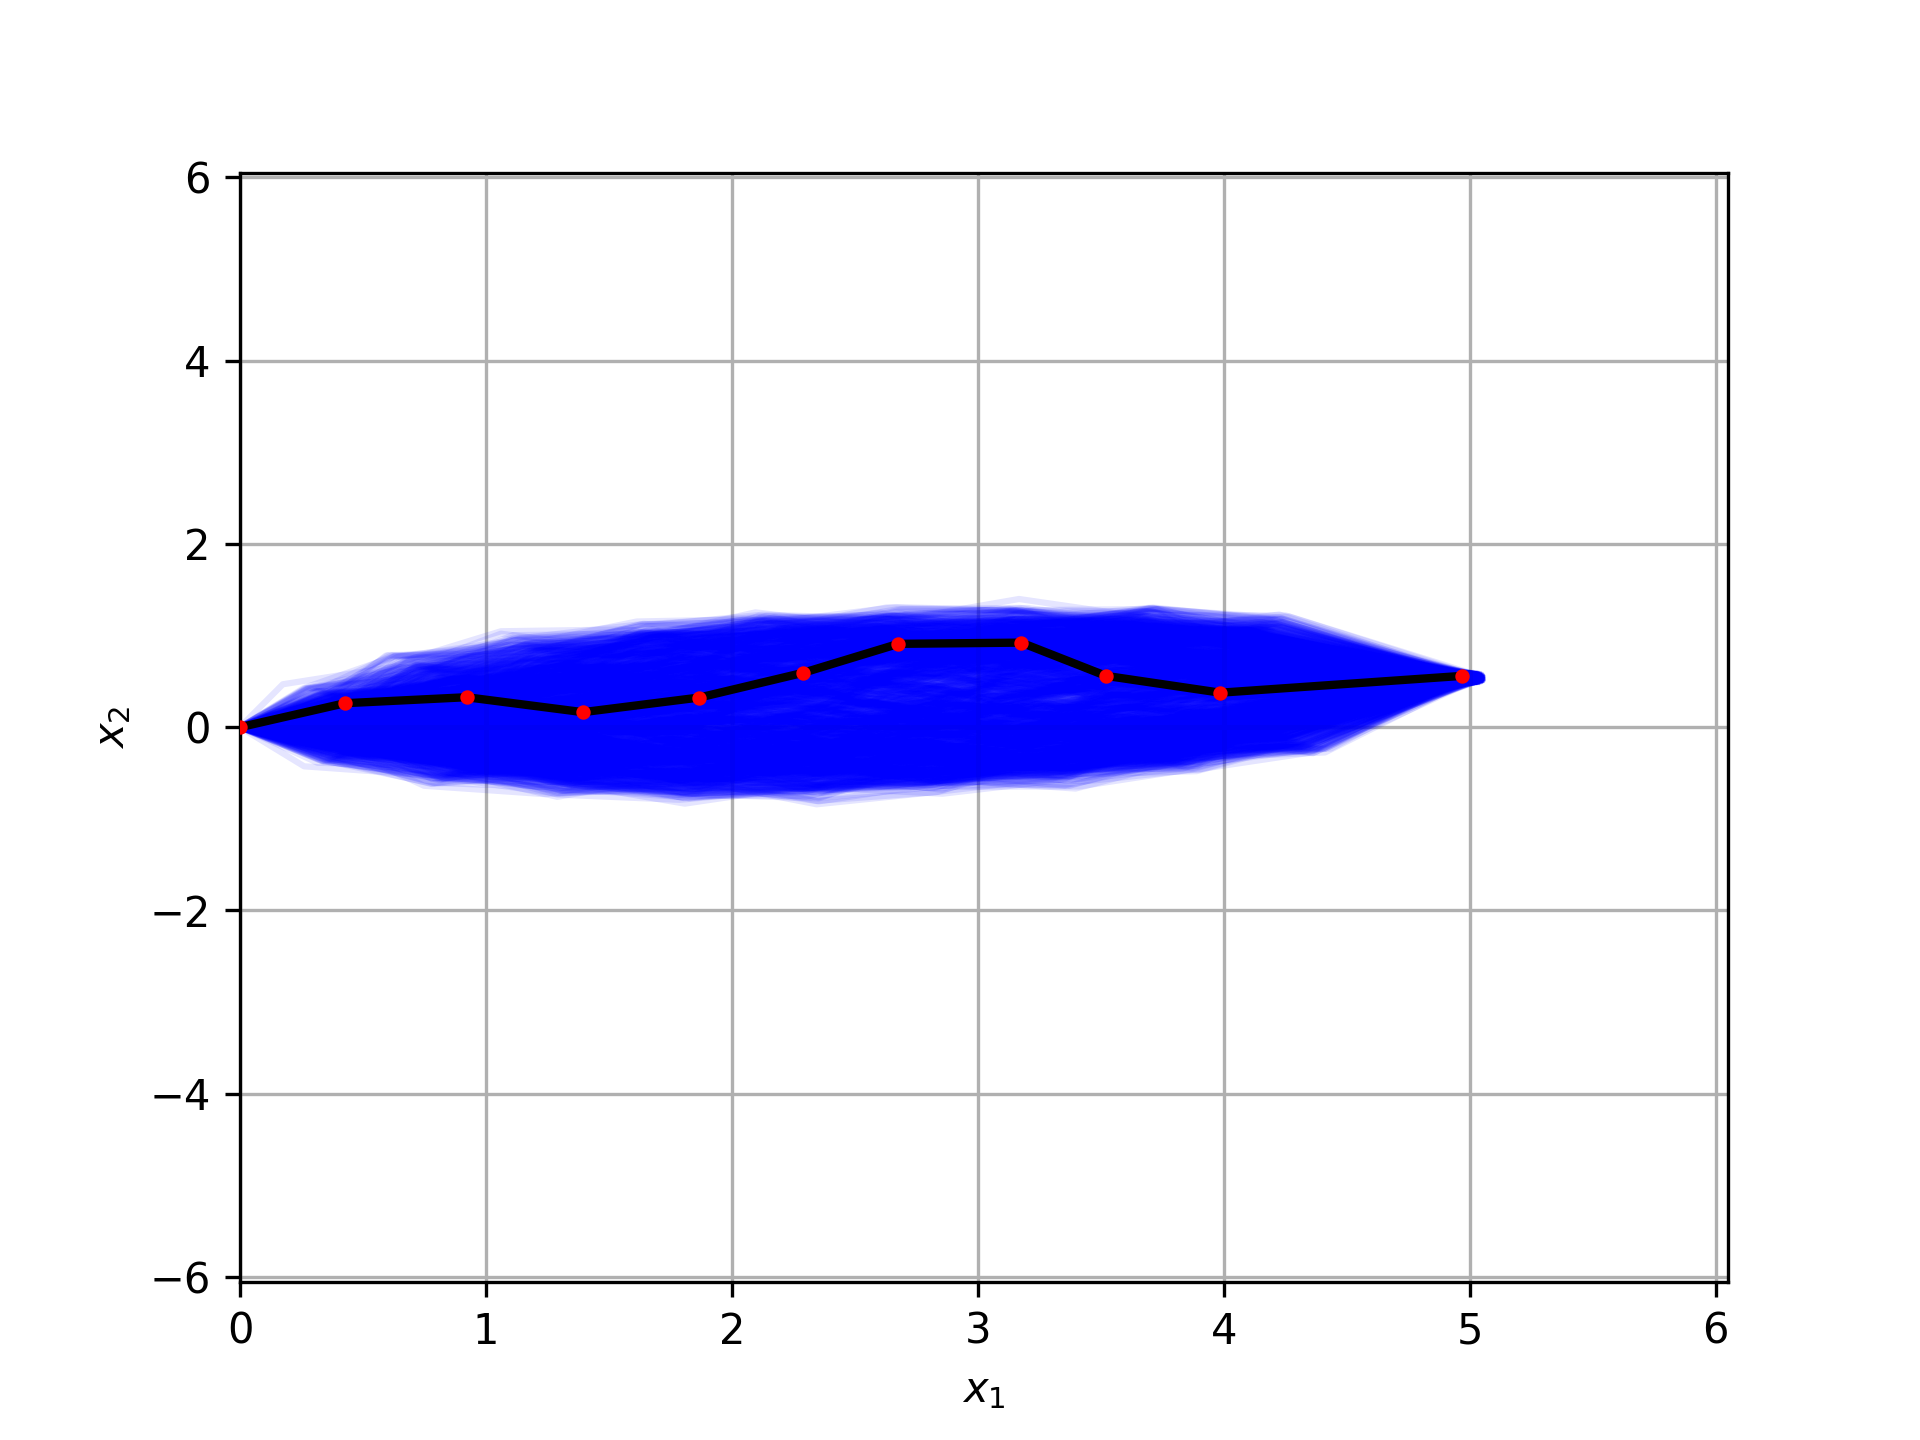
\includegraphics[width=0.32\linewidth]{figures/rejection_sampling_INN_10DOF.png}
    \label{fig:rejection_sampling:10DOF}}
    %
    \subfloat[cVAE]{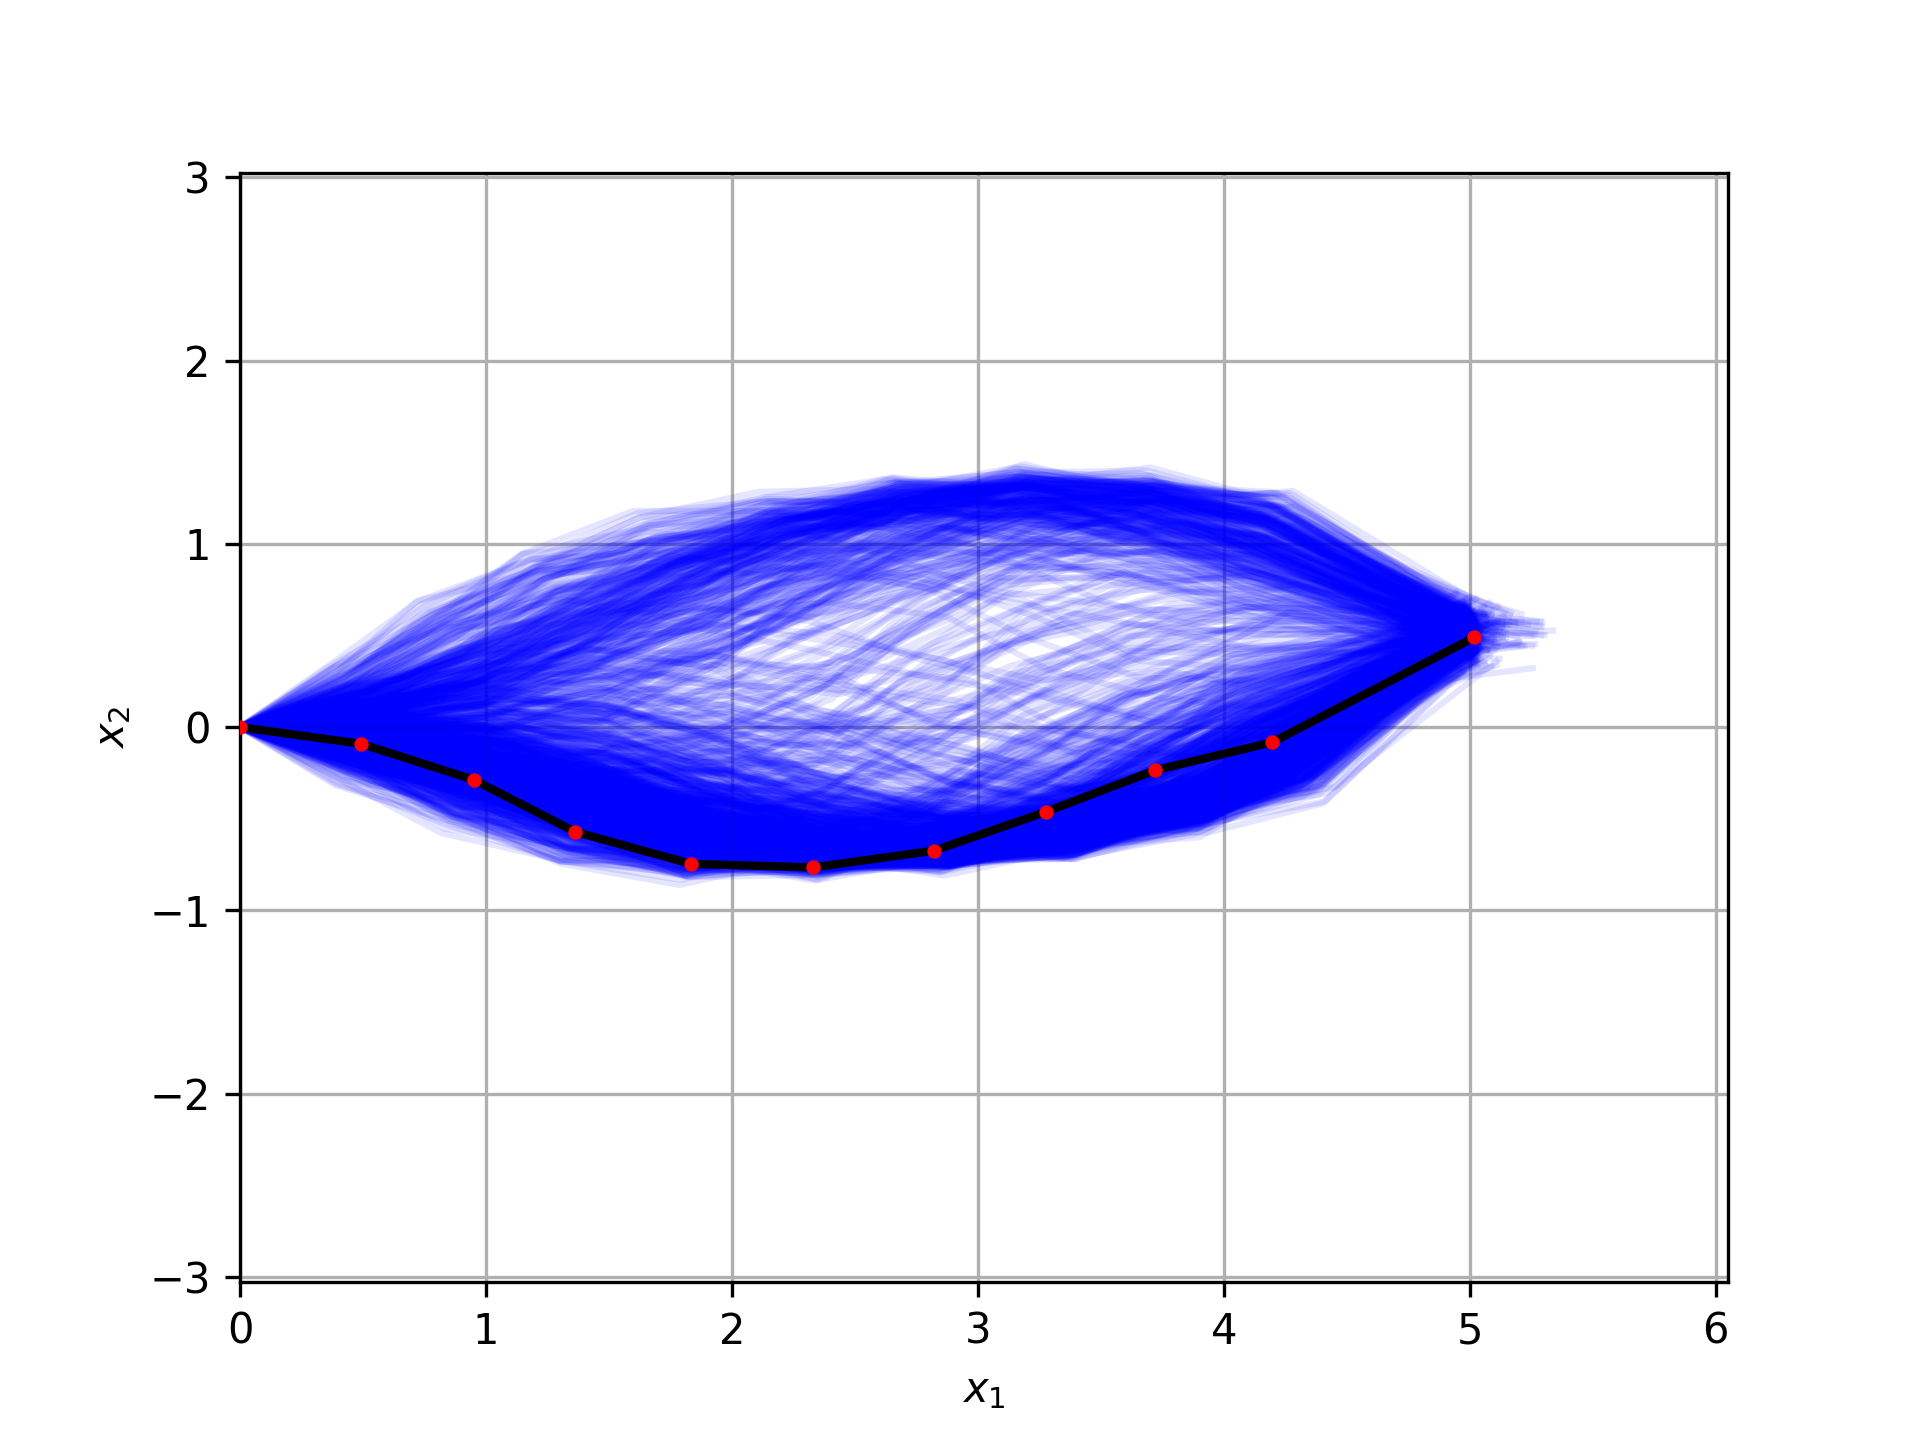
\includegraphics[width=0.32\linewidth]{figures/predicted_posterior_CVAE_10DOF.png}
        \label{fig:cVAE:10DOF}}
    %
    \subfloat[INN]{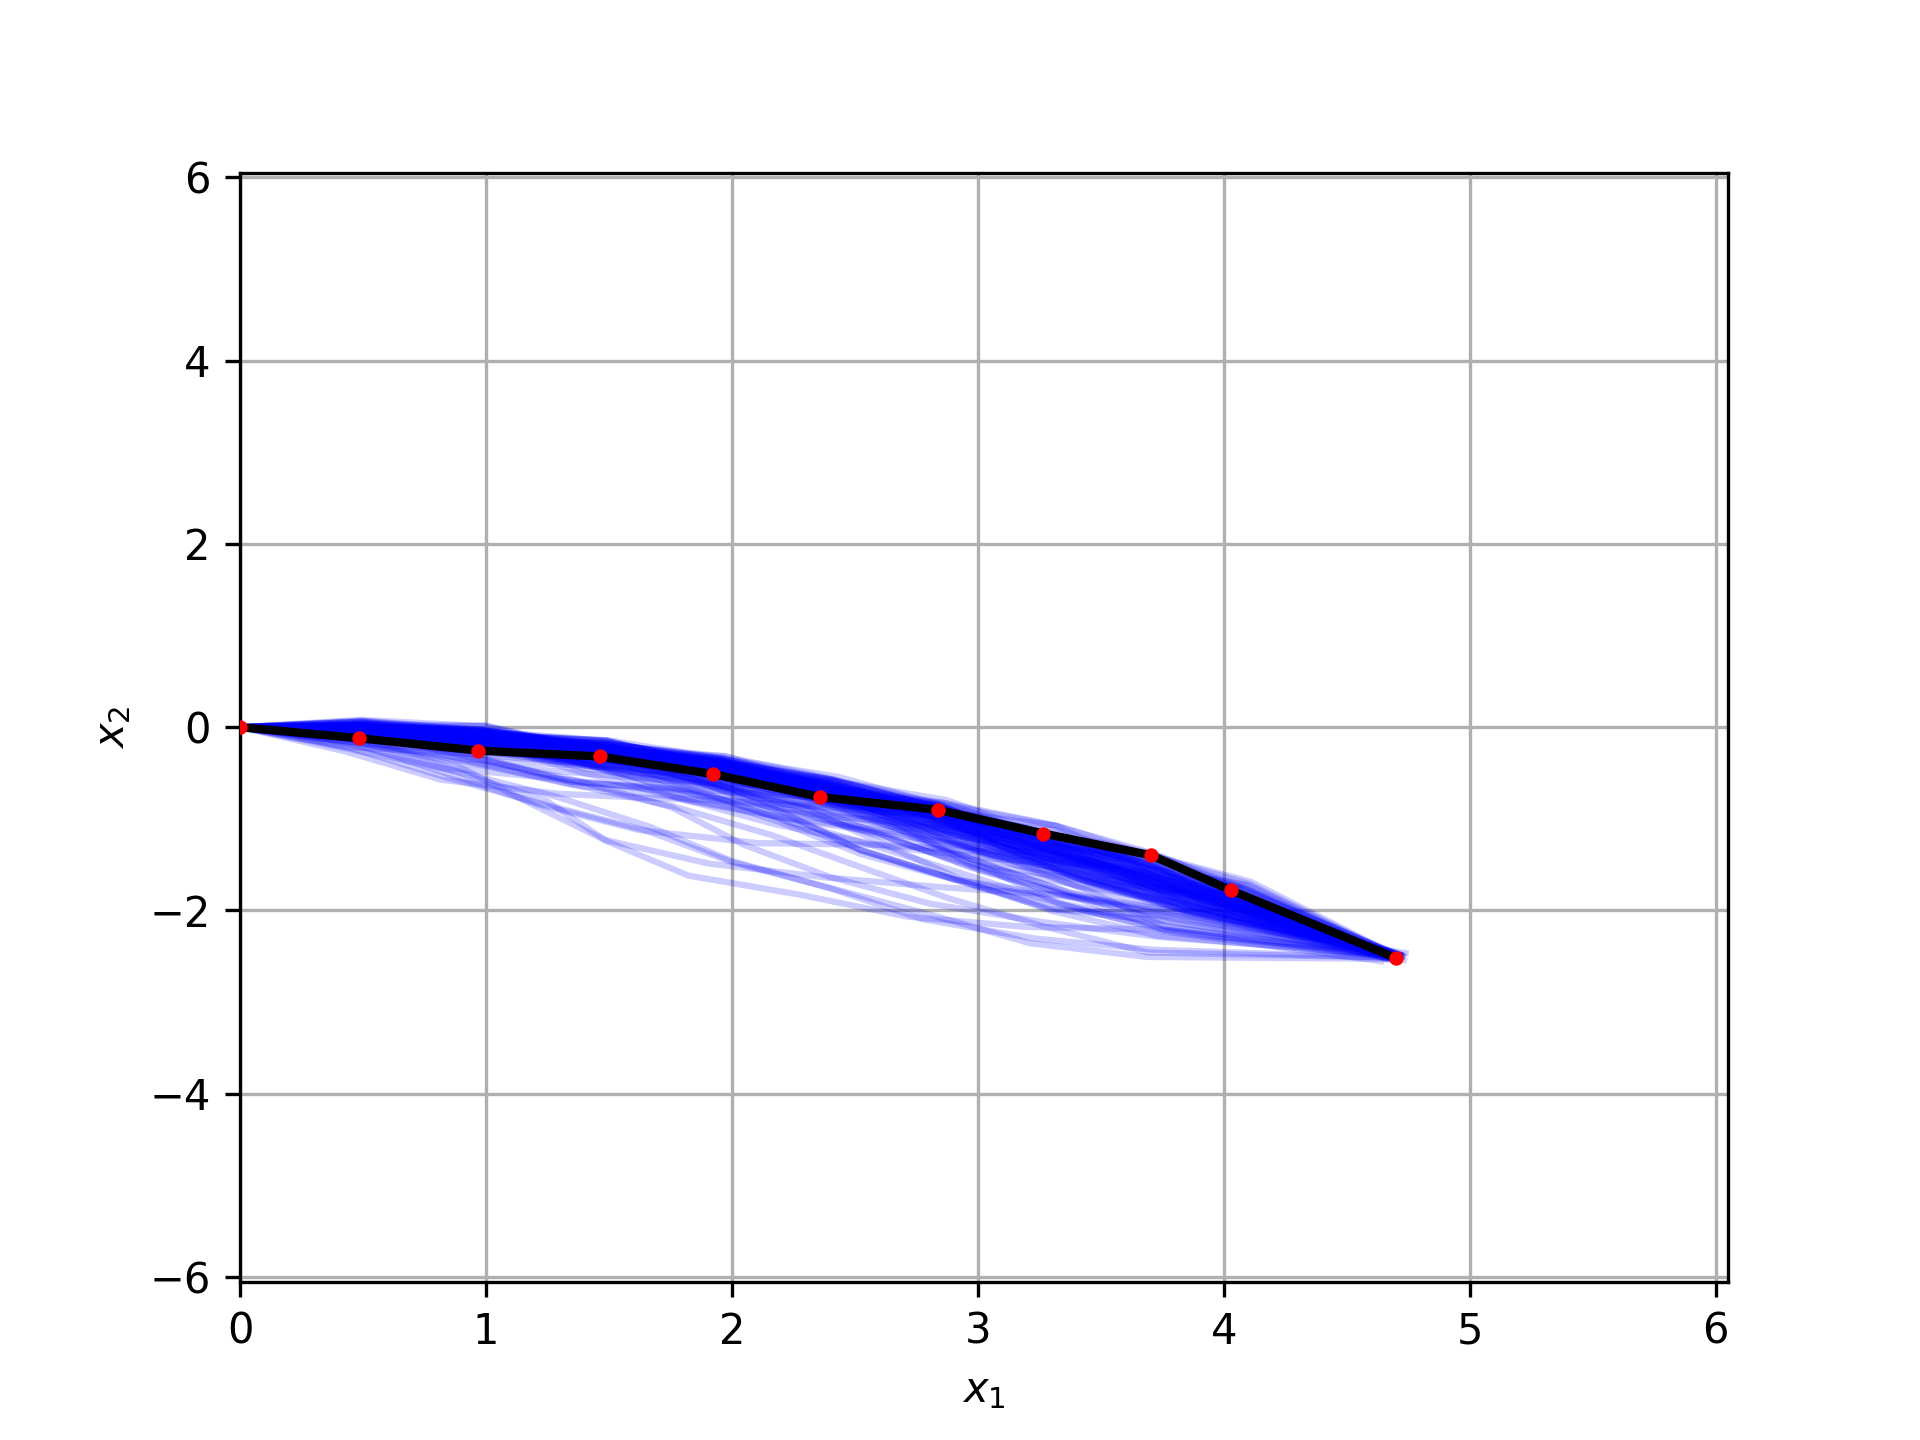
\includegraphics[width=0.32\linewidth]{figures/predicted_posterior_INN_10DOF.png}
        \label{fig:INN:10DOF}}

    \caption{Configurations of a planar manipulator with $10$ revolute joints and end-effector position at $(x, y) = [5.00, 0.53]$. 1000 samples are drawn from each model's predicted posterior $\tilde{p}(x | y_{gt})$. One random sample configuration is highlighted. $e_{posterior} = 0.057$ for the cVAE and $e_{posterior} = 0.025$ for the INN.}
    \label{fig:posterior:10dof}
\end{figure*}

\section*{Conclusion}

In this work, we evaluated the feasibility of using neural networks to learn the posterior distribution of the hidden parameter space in the context of inverse kinematics problems in robotics. For this, we developed simulations of planar robotic arm with an arbitrary number of revolute joints. Using the simulations, we studied Invertible Neural Networks \cite{Ardizzone2018} and compared them to conditional Variational Autoencoders \cite{Sohn2015}. We explored the performance of these architectures for both simple planar robot configurations with 4 revolute joints and more complex configurations with up to 10 revolute joints. To find the best set of hyperparameters we performed a hyperparameter search.

Using evaluation metrics defined in previous research \cite{Kruse2019}, we found that cVAEs are better at predicting the values of the joint angles which result in a given the end-effector position. In contrast, our experiments show that INNs are able to better recover the full posterior distribution over the joint angle space. 

Unlike stated in previous research \cite{Ardizzone2018}, we had to perform an additional unsupervised backward training of the INN to match the performance of the cVAE. This resulted in considerably slower training times for the INN models. Moreover, the INN models tended to be more unstable during training. Despite these shortcomings, INNs are an interesting and powerful tool for recovering the full posterior parameters distribution and also for explicitly computing the posterior probability by using tractable Jacobians.

\nocite{*}
\bibliographystyle{IEEEtran}
\bibliography{IEEEabrv,final_report}

\end{document}
